%
% teil3.tex -- Beispiel-File für Teil 3
%
% (c) 2020 Prof Dr Andreas Müller, Hochschule Rapperswil
%

\section{Anwendung in der Physik 
	\label{parzyl:section:teil2}}
\rhead{Anwendung in der Physik}

Die parabolischen Zylinderkoordinaten tauchen auf, wenn man das elektrische Feld einer semi-infiniten Platte, wie in Abbildung \ref{parzyl:fig:leiterplatte} gezeigt, finden will.
\begin{figure}
	\centering
	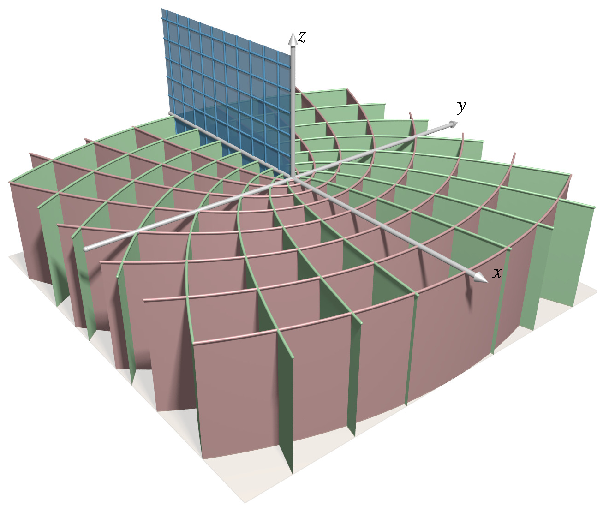
\includegraphics[width=0.8\textwidth]{papers/parzyl/images/halfplane.pdf}
	\caption{Semi-infinite Leiterplatte}
	\label{parzyl:fig:leiterplatte}
\end{figure}
Die Äquipotentiallinien sind dabei in rot ,die des elektrischen Feldes in grün und semi-infinite Platte ist in blau dargestellt.
Das dies so ist kann im Zweidimensionalen mit Hilfe von komplexen Funktionen gezeigt werden. Die Platte ist dann nur eine Halbgerade, was man in Abbildung \ref{parzyl:fig:leiterplatte_2d} sieht.
\begin{figure}
	\centering
	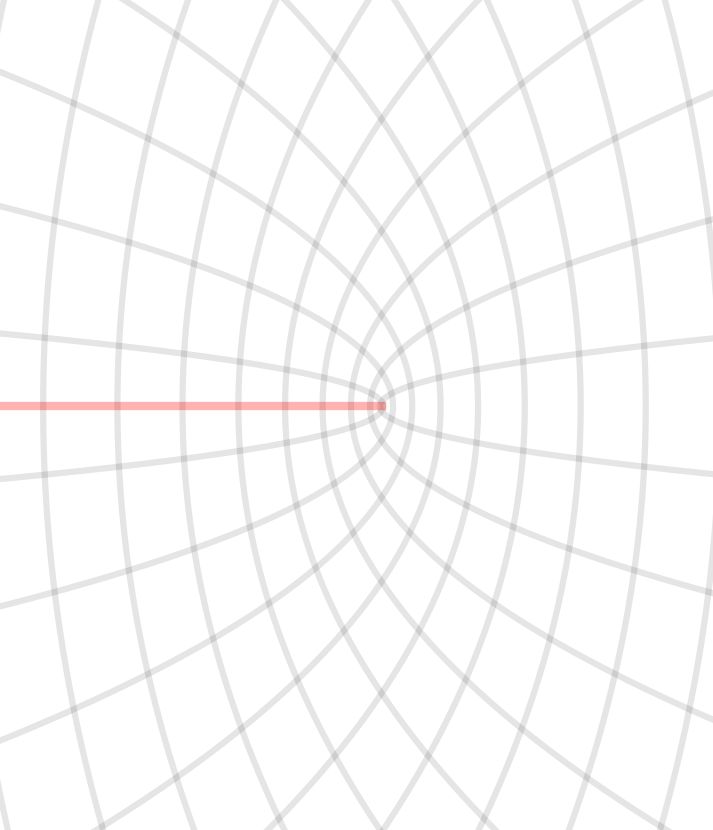
\includegraphics[width=0.6\textwidth]{papers/parzyl/img/Plane_2D.png}
	\caption{Semi-infinite Leiterplatte dargestellt in 2D}
	\label{parzyl:fig:leiterplatte_2d}
\end{figure}

Jede komplexe Funktion $F(z)$ kann geschrieben werden als
\begin{equation}
	F(s) = U(x,y) + iV(x,y) \quad s = x + iy \qquad s \in \mathbb{C}; x,y \in \mathbb{R}.
\end{equation}  
Dabei müssen, falls die Funktion differenzierbar ist, die Cauchy-Riemann Differentialgleichungen 
\begin{equation}
	\frac{\partial U(x,y)}{\partial x} 
	=
	\frac{\partial V(x,y)}{\partial y} 
	\qquad
	\frac{\partial V(x,y)}{\partial x}
	=
	-\frac{\partial U(x,y)}{\partial y}
\end{equation}
gelten.
Aus dieser Bedingung folgt 
\begin{equation}
	\label{parzyl_e_feld_zweite_ab}
	\underbrace{
		\frac{\partial^2 U(x,y)}{\partial x^2}
		+ 
		\frac{\partial^2 U(x,y)}{\partial y^2}
		=
		0
	}_{\displaystyle{\nabla^2U(x,y)=0}}
	\qquad
	\underbrace{
		\frac{\partial^2 V(x,y)}{\partial x^2}
		+
		\frac{\partial^2 V(x,y)}{\partial y^2}
		=
		0
	}_{\displaystyle{\nabla^2V(x,y) = 0}}.
\end{equation}
Zusätzlich kann auch gezeigt werden, dass die Funktion $F(z)$ eine winkeltreue Abbildung ist.


Der Zusammenhang zum elektrischen Feld ist jetzt, dass das Potential an einem quellenfreien Punkt gegeben ist als 
\begin{equation}
	\nabla^2\phi(x,y) = 0.
\end{equation}
Dies ist eine Bedingung, welche differenzierbare Funktionen, wie in Gleichung \eqref{parzyl_e_feld_zweite_ab} gezeigt wird, bereits besitzen. 


Nun kann zum Beispiel $U(x,y)$ als das Potential angeschaut werden:
\begin{equation}
	\phi(x,y) = U(x,y).
\end{equation}
Orthogonal zu den Äquipotenzialflächen sind die Feldlinien des elektrische Feld
\begin{equation}
	E(x,y) = V(x,y).
\end{equation}


Um nun zu den parabolische Zylinderkoordinaten zu gelangen, muss nur noch eine geeignete 
komplexe Funktion $F(s)$ gefunden werden, 
welche eine semi-infinite Platte beschreiben kann.


Die gesuchte Funktion in diesem Fall ist
\begin{equation}
	F(s) 
	= 
	\sqrt{s} 
	= 
	\sqrt{x + iy}.
\end{equation}
Dies kann umgeformt werden zu
\begin{equation}
	F(s) 
	= 
	\underbrace{\sqrt{\frac{\sqrt{x^2+y^2} + x}{2}}}_{U(x,y)} 
	+ 
	i\underbrace{\sqrt{\frac{\sqrt{x^2+y^2} - x}{2}}}_{V(x,y)}
	.
\end{equation}


%Die Äquipotentialflächen können nun betrachtet werden, 
%indem man die Funktion, welche das Potential beschreibt, gleich eine Konstante setzt,
%\begin{equation}
%	\sigma = U(x,y) = \sqrt{\frac{\sqrt{x^2+y^2} + x}{2}}.
%\end{equation}
%Die Flächen mit der gleichen elektrischen Feldstärke können als
%\begin{equation}
%	\tau = V(x,y) = \sqrt{\frac{\sqrt{x^2+y^2} - x}{2}}
%\end{equation}
%beschrieben werden. Diese zwei Gleichungen zeigen nun, wie man vom 
%kartesischen Koordinatensystem ins parabolische Zylinderkoordinatensystem kommt.

Die Äquipotentialflächen können nun betrachtet werden, 
indem man die Funktion, welche das Potential beschreibt, gleich eine Konstante setzt,
\begin{equation}
%	\sigma = U(x,y) = \sqrt{\frac{\sqrt{x^2+y^2} + x}{2}}.
	c_1 = U(x,y) = \sqrt{\frac{\sqrt{x^2+y^2} + x}{2}}.
\end{equation}
Die Flächen mit der gleichen elektrischen Feldstärke können als
\begin{equation}
%	\tau = V(x,y) = \sqrt{\frac{\sqrt{x^2+y^2} - x}{2}}
	c_2 = V(x,y) = \sqrt{\frac{\sqrt{x^2+y^2} - x}{2}}
\end{equation}
beschrieben werden. Diese zwei Gleichungen zeigen nun, wie man vom 
kartesischen Koordinatensystem ins parabolische Zylinderkoordinatensystem kommt.
%Werden diese Formeln nun nach $x$ und $y$ aufgelöst 
%\begin{equation}
%	x = \sigma \tau,
%\end{equation}
%\begin{equation}
%	y = \frac{1}{2}\left ( \tau^2 - \sigma^2 \right ),
%\end{equation}
%so beschreibe sie, wie man aus dem parabolischen Zylinderkoordinatensystem zurück ins kartesische rechnen kann.
Werden diese Formeln nun nach $x$ und $y$ aufgelöst 
\begin{align}
	x &=  c_1^2 - c_2^2 ,\\
	y &= 2c_1 c_2,
\end{align}
so beschreiben sie mit $\tau = c_1 \sqrt{2}$ und $\sigma = c_2 \sqrt{2}$ die Beziehung 
zwischen dem parabolischen Zylinderkoordinatensystem und dem kartesischen Koordinatensystem.

Nun wurde gezeigt wieso sich das parabolische Zylinderkoordinatensystem am besten eignet um das Potential und das elektrische Feld einer semi-infiniten Leiterplatte zu beschreien. Falls man nun die Helmholtz-Gleichung in diesem Bereich lösen müsste, da man zum Beispiel am Verhalten einer elektromagnetischne Welle in der Nähe der Platte interessiert wäre, so würde man auf die parabolischen Zylinderfunktionen kommen. 
%Werden diese Formeln nun nach $x$ und $y$ aufgelöst 
%\begin{equation}
%	x = \sigma \tau,
%\end{equation}
%\begin{equation}
%	y = \frac{1}{2}\left ( \tau^2 - \sigma^2 \right ),
%\end{equation}
%so beschreibe sie, wie man aus dem parabolischen Zylinderkoordinatensystem zurück ins kartesische rechnen kann.